\documentclass[tikz,border=6pt]{standalone}
\usepackage{tikz}
\usetikzlibrary{arrows.meta}
\definecolor{nebula}{HTML}{6366F1}
\definecolor{spark}{HTML}{14B8A6}
\definecolor{ink}{HTML}{334155}
\begin{document}
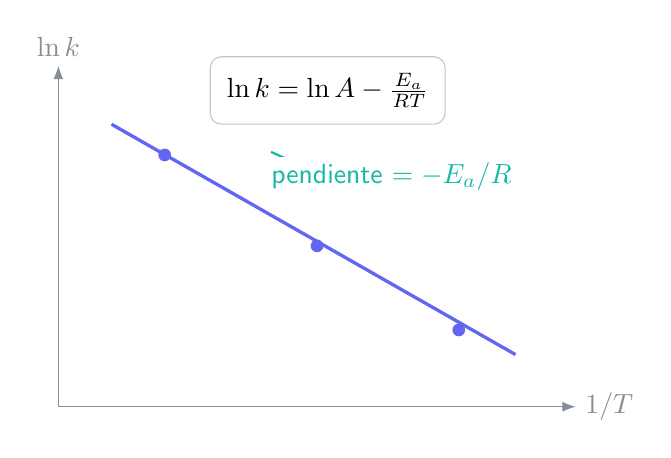
\begin{tikzpicture}[font=\sffamily,>=Latex,x=.9cm,y=.78cm]
  \draw[->,ink!60] (0,0)--(7.3,0) node[right] {$1/T$};
  \draw[->,ink!60] (0,0)--(0,5.55) node[above] {$\ln k$};
  \draw[very thick,nebula] (.75,4.6)--(6.45,.85);
  \fill[nebula] (1.5,4.1) circle (2.3pt);
  \fill[nebula] (3.65,2.62) circle (2.3pt);
  \fill[nebula] (5.65,1.25) circle (2.3pt);
  \draw[->,thick,spark] (3.0,4.15)--(4.35,3.45);
  \node[text=spark,fill=white,inner sep=2pt] at (4.7,3.75) {pendiente $=-E_a/R$};
  \node[draw=ink!30,rounded corners=4pt,fill=white,inner sep=6pt] at (3.8,5.15) {$\ln k=\ln A-\frac{E_a}{RT}$};
\end{tikzpicture}
\end{document}
